\documentclass[../main.tex]{subfiles}
\begin{document}

\subsection{Project background}
\label{sec:project-background}

In recent years, \gls{dl} has significantly improved the
performance of a wide range of computer vision tasks like image classification,
object detection or semantic segmentation.
\gls{gans} in particular have revolutionized generative tasks like image synthesis
and image-to-image translation.
Image-to-image translation is the task of generating an image based on a
given source image with different characteristics depending on the specific problem.

In this project, based on \parencite{Combalia2019} work in the Dermatology
Department from the \gls{hc},
the idea of image-to-image translation
is applied to the transformation of \gls{cm} images into images with the
appearance of \gls{he} images.

\subsubsection{Confocal microscopy}
\gls{cm} is an optical imaging technique for increasing optical resolution
and contrast of a micrograph by means of using a spatial pinhole to block
out-of-focus light in image formation. With it, technicians are able to slice
thin sections out of thick fluorescent specimens, view specimens
in planes tilted to the line of sight, penetrate deep into light-scattering
tissues or obtain 3D views at very high resolution (\cite{Inoue2006}).

Ex vivo\footnote{Ex vivo means that which takes place outside an organism.
In science, ex vivo refers to experimentation or measurements done in or on
tissue from an organism in an external environment with minimal alteration
of natural conditions.} confocal scanning laser microscopy can potentially
accelerate Mohs surgery\footnote{Mohs micrographic surgery is considered the
most effective technique for treating many basal cell carcinomas (BCCs) and
squamous cell carcinomas (SCCs), the two most common types of skin cancer.
The procedure is done in stages, including lab work, while the patient waits.
This allows the removal of all cancerous cells for the highest cure rate
while sparing healthy tissue and leaving the smallest possible scar.}
by rapidly detecting carcinomas without conventional frozen histopathology
(and its consequential time delays) (\cite{Chung2005}).

Two different \gls{cm} modes exist, \gls{rcm} displays the backscattering signal
of naturally occurring skin components, whereas \gls{fcm} provides contrast
by using an applied fluorescent dye (\cite{Skvara2012}).
See figure \ref{fig:CM-example} for an example.

\begin{figure}[h]
\centering
\begin{subfigure}{.5\textwidth}
  \centering
  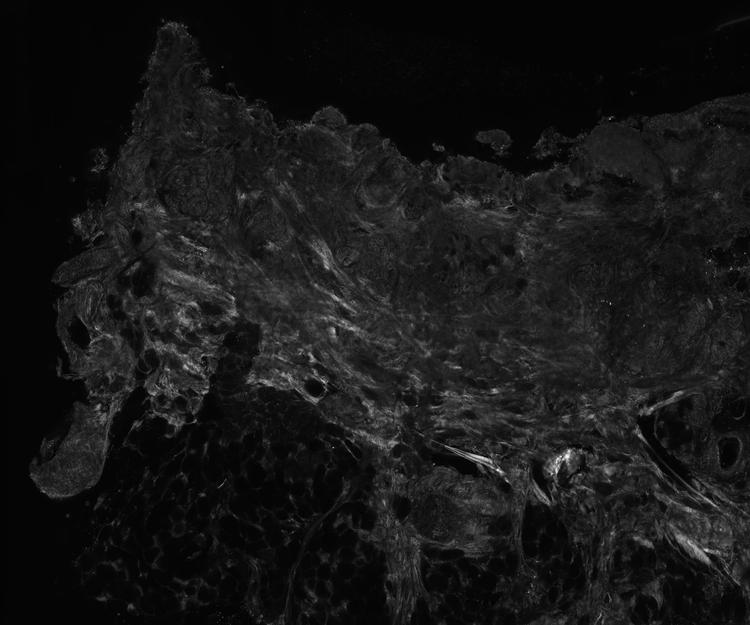
\includegraphics[width=.8\linewidth]{R_crop_thumbnail}
  \label{fig:R-example}
\end{subfigure}%
\begin{subfigure}{.5\textwidth}
  \centering
  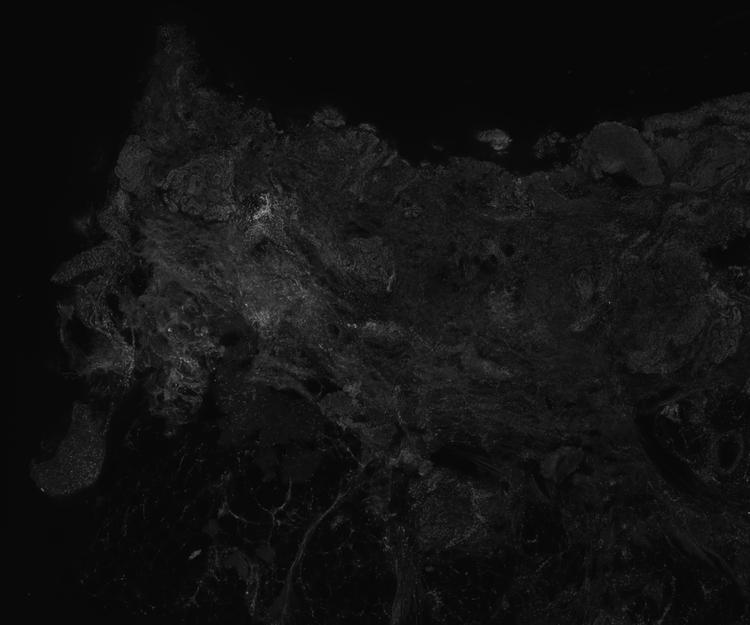
\includegraphics[width=.8\linewidth]{F_crop_thumbnail}
  \label{fig:F-example}
\end{subfigure}
\caption{Example of a CM micrograph of a skin tissue.
Reflectance mode on the left and fluorescence mode on the right}
\label{fig:CM-example}
\end{figure}

\subsection{Problem statement}
\label{sec:problem-statement}
\gls{cm} has enabled rapid evaluation of tissue samples
directly in the surgery room significantly reducing the time of complex
surgical operations in skin cancer (\cite{Cinotti2018}),
but the output largely differs from the standard \gls{he} slides that
pathologists typically use to analyze tissue samples.
See figure \ref{fig:HE-example} for a \gls{he} example.

To bridge this gap, a method for combining the aforementioned modes of
\gls{cm} into a H\&E-like image is presented in this work.
A correctly done CM to H\&E mapping would bring the efficiency of \gls{cm}
to untrained pathologists and surgeons.

Similar to a false color (also known as pseudo color) transformation,
a parametric mapping function can be defined:
\begin{equation} \label{eq:mapping-function}
	\tensor{DSCM}
	= f_{\theta}(\tensor{R}, \tensor{F})
\end{equation}
where $\tensor{DSCM} \in \R{}^{H \times W \times 3}$ (stands for digitally-stained
\gls{cm}) represents the resulting H\&E-like RGB image,
$\tensor{R}, \tensor{F} \in \R{}^{H \times W}$
represent the reflectance and fluorescence modes (respectively) of the \gls{cm} input
image with height $H$ and width $W$.

\subsubsection{Affine transformation} \label{sec:affine-transformation}
\definecolor{Hcolor}{rgb}{0.3,0.2,1}
\definecolor{Ecolor}{rgb}{1,0.55,0.88}
A color affine transfomation is proposed in \parencite{Gareau2009} for the
function $f$
where the RGB values for each pixel are computed as:
\begin{equation} \label{eq:affine-transformation}
	\tensor{DSCM}_{x,y} = \tensor{1}
	- \text{F}_{x,y} (\tensor{1} - \tensor{H}) - \text{R}_{x,y} (\tensor{1} - \tensor{E})
\end{equation}
where:
\begin{align*}
\tensor{H} &= \begin{bmatrix} 0.30 & 0.20 & 1 \end{bmatrix} \\
\tensor{E} &= \begin{bmatrix} 1 & 0.55 & 0.88 \end{bmatrix}
\end{align*}
$\tensor{H}$ and $\tensor{E}$ vectors represent color coordinates in the RGB
space (
\textcolor{Hcolor}{\rule{0.7\baselineskip}{0.7\baselineskip}} and
\textcolor{Ecolor}{\rule{0.7\baselineskip}{0.7\baselineskip}}).
This way, the transformed \gls{cm} modes highlight different structures in
distinct
colours similar to a \gls{he} slide. However, as it can be seen in figure
\ref{fig:affine-example},
the color scheme differs from an actual \gls{he} sample.

\begin{figure}[h]
\centering
\begin{subfigure}{.5\textwidth}
  \centering
  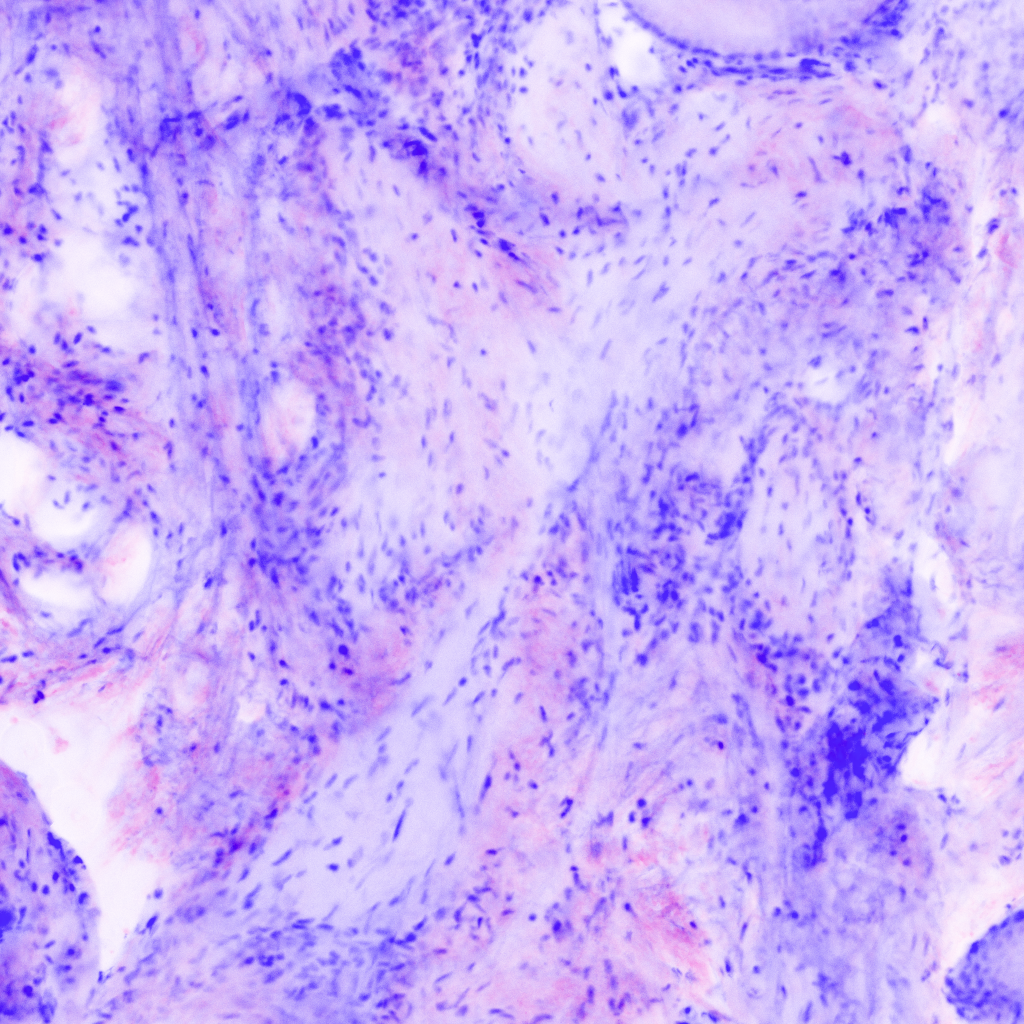
\includegraphics[width=.8\linewidth]{DSCM_Gareau}
  \caption{Digitally stained sample using the affine transformation of equation
  \eqref{eq:affine-transformation}}
\end{subfigure}%
\begin{subfigure}{.5\textwidth}
  \centering
  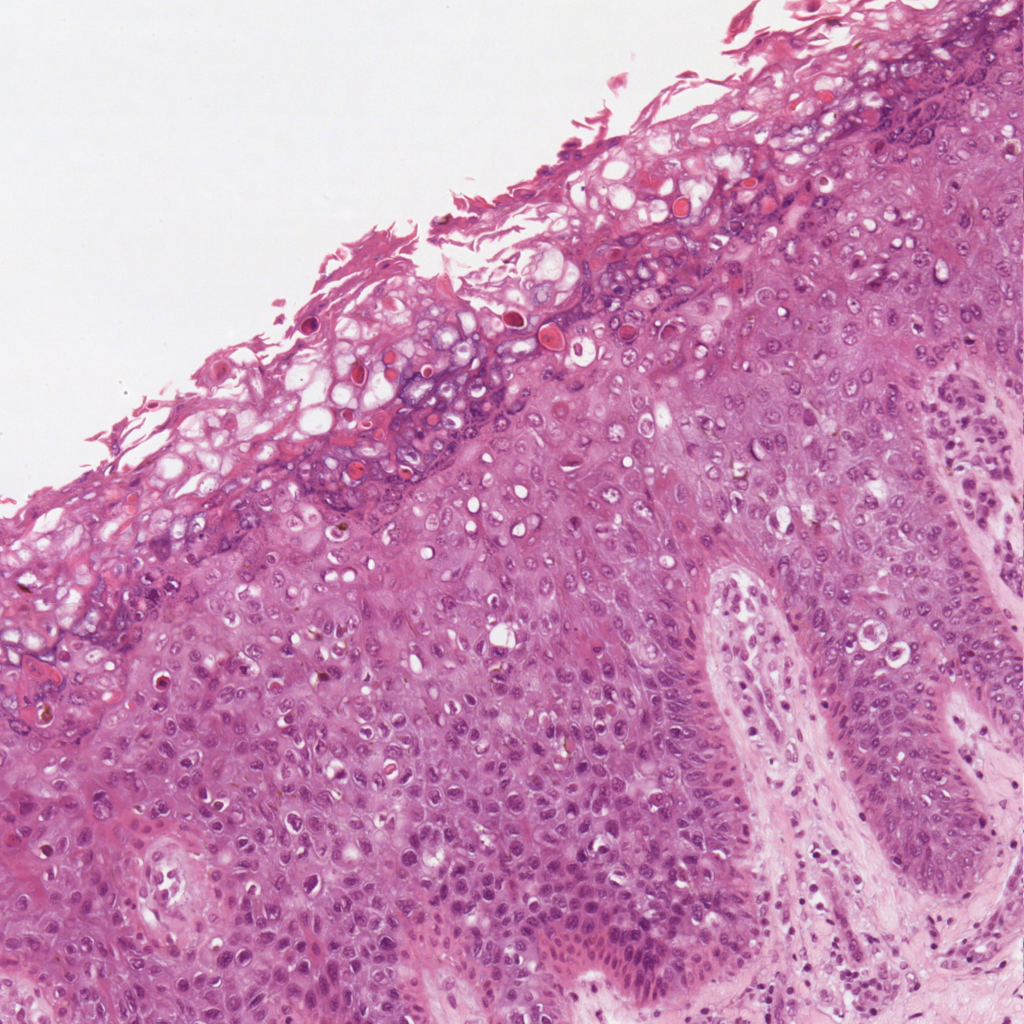
\includegraphics[width=.8\linewidth]{HE}
  \caption{H\&E stained sample}
  \label{fig:HE-example}
\end{subfigure}
\caption{Comparison between digital stain and H\&E stain}
\label{fig:affine-example}
\end{figure}

\subsubsection{Data-driven approach}
In contrast to \parencite{Gareau2009}, work where the parameters
($\tensor{H}$ and $\tensor{E}$) are found experimentally, a data-driven approach
of the problem will be taken where the parameters of the mapping function
\eqref{eq:mapping-function} will be \emph{learned} based on data.
More specifically, the transformation will be defined by a \gls{nn} (called \emph{StainNN})
and the parameters will be searched through an adversarial setting.

\subsubsection{Speckle noise reduction}\label{sec:speckle-noise}
\gls{rcm} images are affected by a multiplicative noise known as speckle,
which may impair the performance of post-processing techniques.
Hence, before digitally staining the \gls{cm} images, this noise must be reduced.

The observed \gls{rcm} image $Y$ is related to the noise free image $X$ by
the following multiplicative model:
\begin{equation} \label{eq:speckle-model}
	Y = X \odot F
\end{equation}
Where $\odot$ denotes the Hadamard product (also known as the elementwise product)
and $F$ is the speckle noise random variable.

To reduce the speckle noise, a data-driven approach will also be taken using
a neural network called \emph{DespecklingNN}.

\subsection{Methods and procedures}
\label{sec:methods-and-procedures}
This project was carried out at the Image and Video Processing Group (GPI) research
group from the Signal Theory and Communications Department (TSC) at the Universitat
Politecnica de Catalunya (UPC) in collaboration with the Dermatology Department from
the Hospital Clínic de Barcelona.

The work presented in this thesis is the natural continuation of the work presented
in \parencite{Combalia2019}.

All the experiments are implemented with Python using the following
libraries\footnotemark:
\begin{itemize}
\item \href{https://numpy.org/}{NumPy} for general purpose data manipulation.
\item \href{https://pytorch.org/}{PyTorch} for training and using \gls{dl} models.
\item \href{https://libvips.github.io/libvips/}{pyvips} for processing big image files.
\item \href{https://scikit-image.org/}{scikit-image} for image manipulation.
\item \href{https://seaborn.pydata.org/}{seaborn} for data visualization.
\end{itemize}

\footnotetext{Private git repository with most of the scripts at
\url{https://github.com/imatge-upc/Confocal}}

\subsection{Document structure}
In section \ref{sec:theoric-background} an overview of relevant \gls{dl} techniques and algorithms
is presented to provide the reader a general knowledge of the field.

Section \ref{sec:methodology} contains the methodology of the project with detailed
explanations of the models used to solve the presented problems. First the
\emph{DespeklingNN} is introduced in \ref{sec:despeckling-network} then the
\emph{StainNN} in \ref{sec:stain-network}.

The experiments carried out to choose the right models are presented in section
\ref{sec:experiments-and-results}.

Finally, the conclusions and future work are discused in section
\ref{sec:conclusions-and-future-development}.
\end{document}
